\subsection{Pulse width calibration}
\label{subsec:poise__pulsecal}

The first of these applications is the calibration of a \ang{90} \proton{} pulse, which is applicable to virtually every NMR experiment.
Essentially, we seek to determine $\taup$ for which
\begin{equation}
    \label{eq:pw90}
    \taup \omega_1 = \frac{\pi}{2},
\end{equation}
where the RF amplitude $\omega_1$ is not known \textit{a priori} (it is only indirectly controlled via the power level).
This pulse width is conventionally specified as the \texttt{P1} parameter in TopSpin.

\subsubsection{Optimisation setup}

In theory, performing a pulse--acquire spectrum with a perfect \ang{180} or \ang{360} pulse would yield no detectable (i.e.\ transverse) magnetisation, i.e.\ a \textit{null}.
Generally, the \ang{360} null is preferred as it minimises effects due to radiation damping, and also allows a smaller recovery delay to be used.
We can use POISE to search for this by acquiring the spectrum, performing a magnitude-mode calculation, and using the intensity of the resulting spectrum as a cost function:
\begin{equation}
    \label{eq:minabsint}
    f_{\symup{m}\text{inabsint}} = \sum_i |S_i|,
\end{equation}
where (reusing notation from \cref{subsec:pureshift__optim_techniques}) $\symbf{S}$ is the spectrum under consideration represented as a complex-valued vector, and the $i$-th point of the spectrum is $S_i = \sqrt{\symbf{S}_{\text{re},i}^2 + \symbf{S}_{\text{im},i}^2}$.
The label \texttt{minabsint} refers to how this cost function drives the optimisation to \textit{min}imise the \textit{abs}olute \textit{int}ensity of the spectrum.
To show how easily this can be coded in Python 3, an implementation of this is shown in \cref{lst:minabsint} (for all other cost functions in this chapter, the reader is directed to the POISE source code for their implementations).
The \texttt{get1d\_...} helper functions are provided by POISE.

\begin{mylisting}[htb]
\begin{tcbminted}{python}
def minabsint():
    r = get1d_real()
    i = get1d_imag()
    mag = np.abs(r + 1j * i)
    return np.sum(mag)
\end{tcbminted}
\caption[Implementation of \texttt{minabsint} cost function]{The implementation of the \texttt{minabsint} cost function in POISE.}
\label{lst:minabsint}
\end{mylisting}

\begin{figure}[htb]
    \centering
    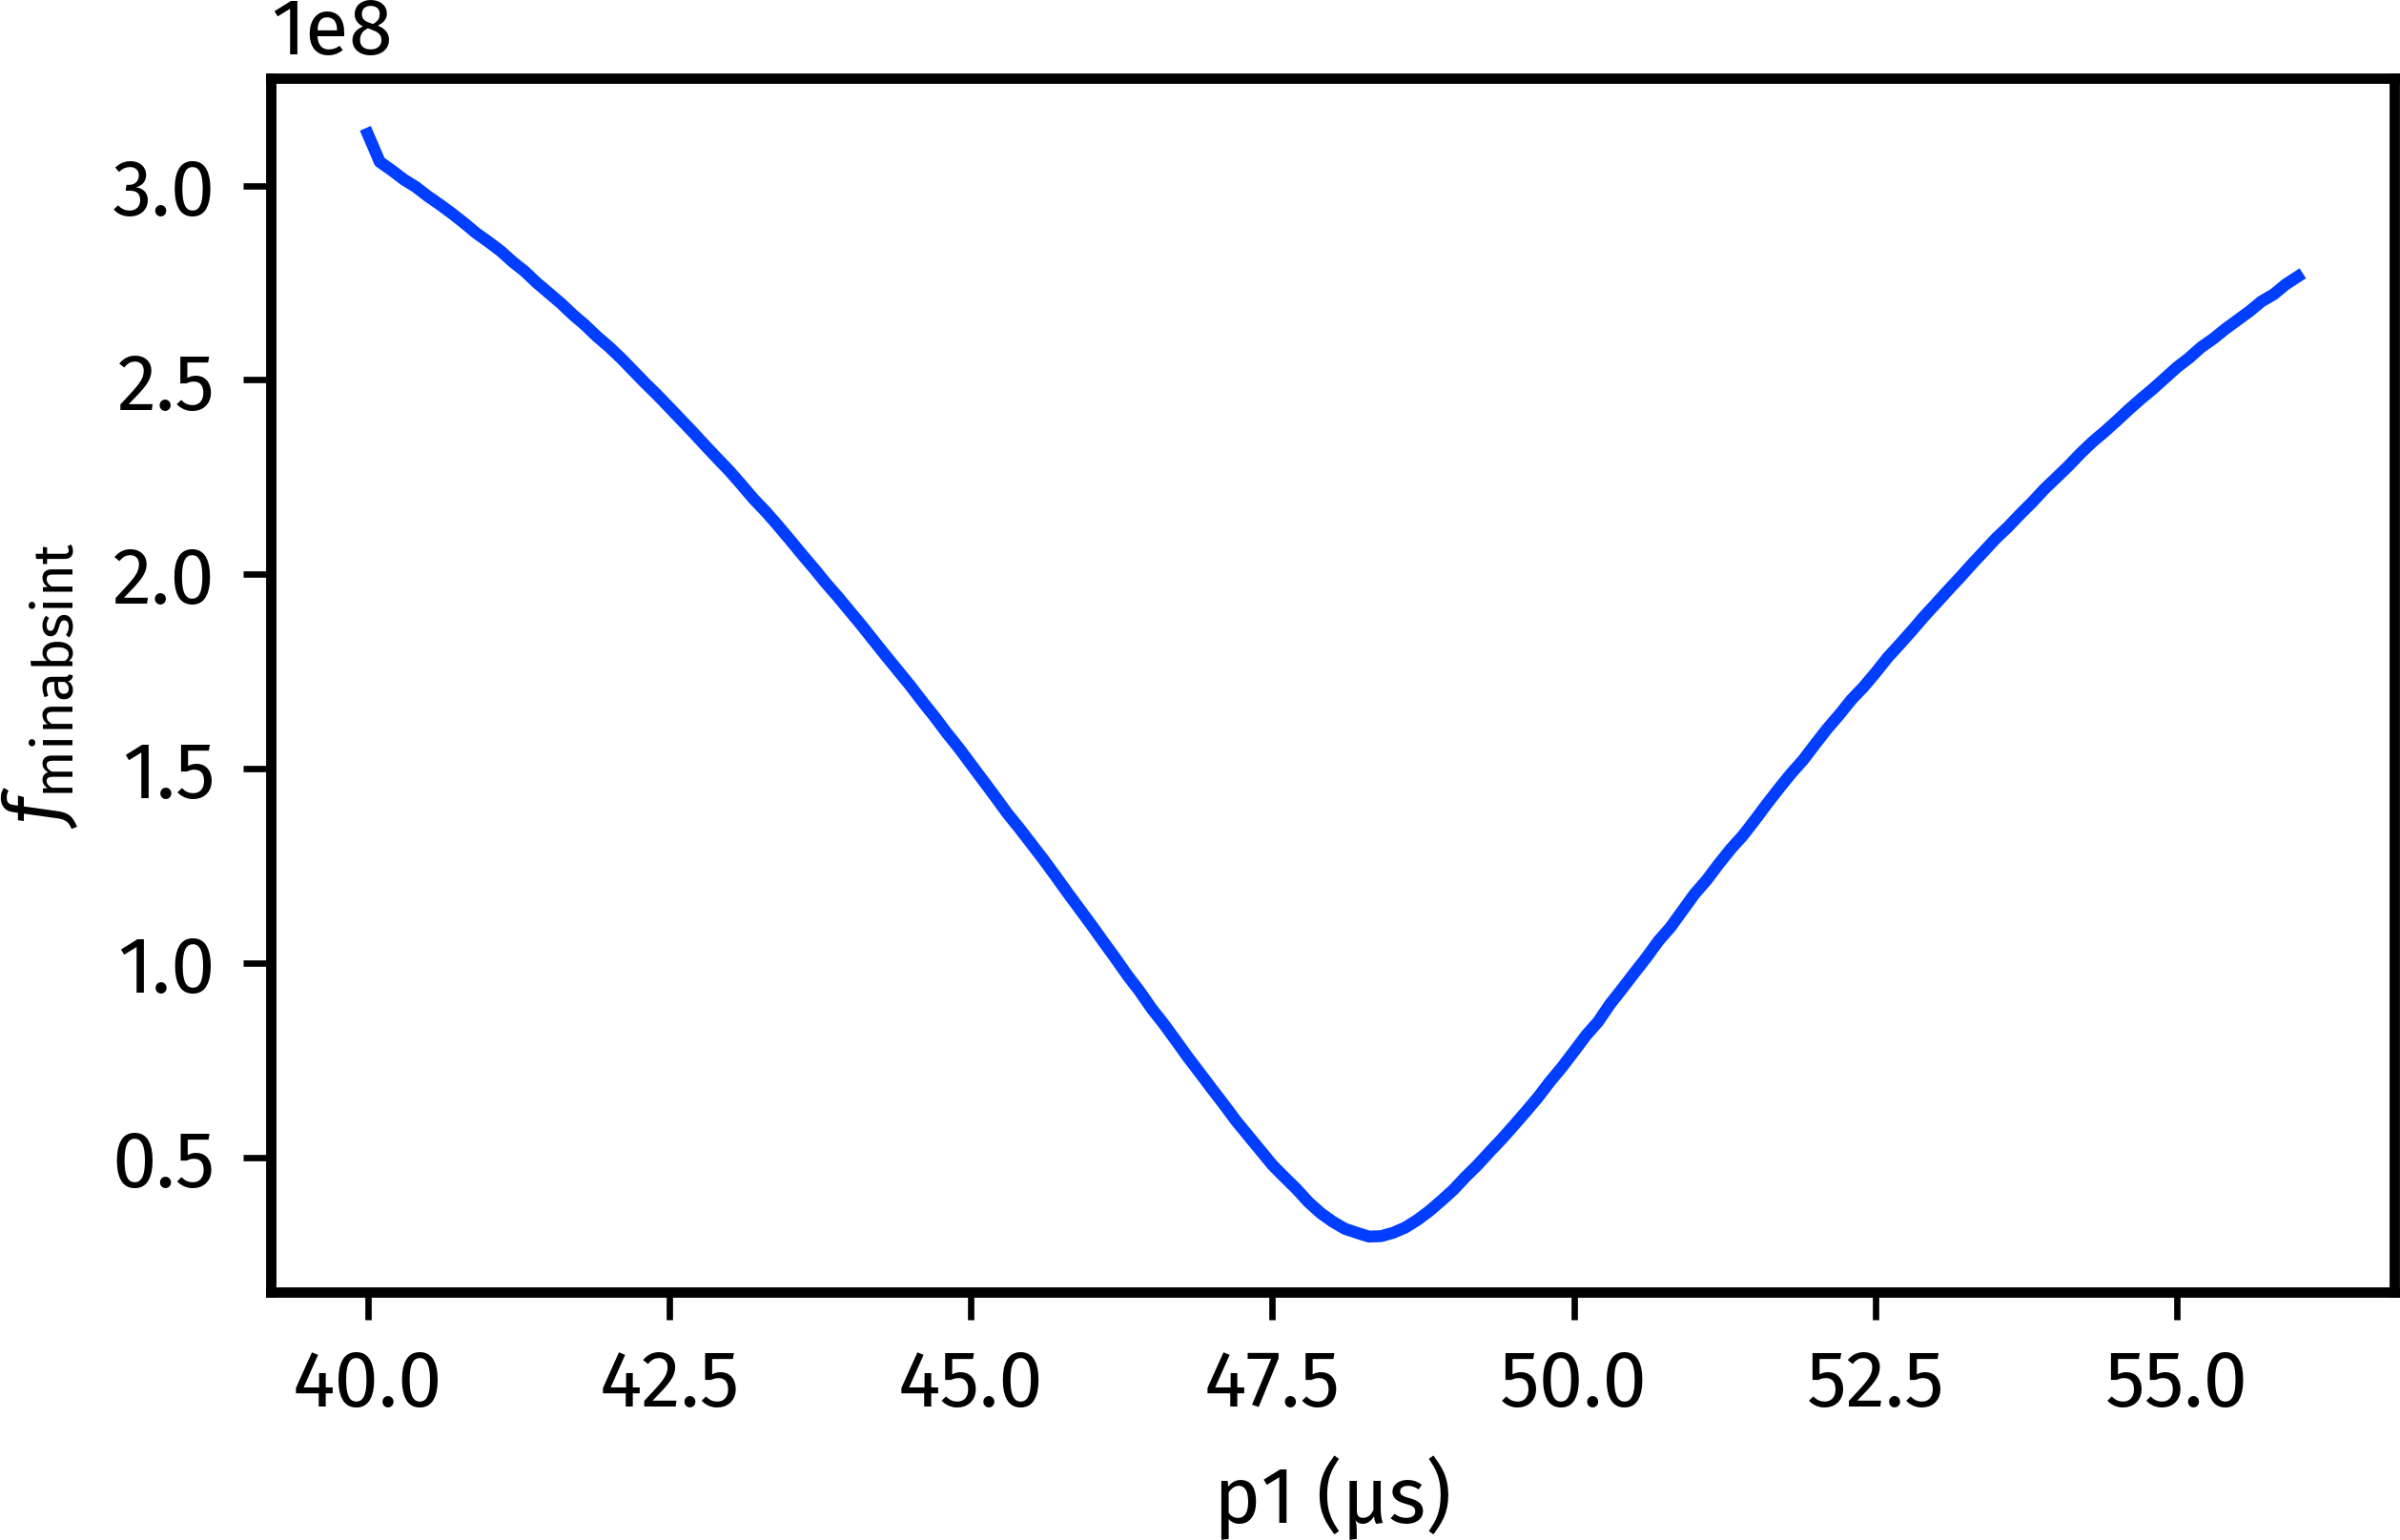
\includegraphics[]{poise/p1_scan.png}%
    \caption[Reference grid search for pulse width optimisation]{
        Reference grid search, showing how the \texttt{minabsint} cost function varies with the pulse width \texttt{P1}.
        \datacode{6F-200826}
    }
    \label{fig:p1_scan}
\end{figure}

To check whether this cost function was sensible, I manually acquired a series of spectra with increasing pulse widths and calculated $f_{\symup{m}\text{inabsint}}$ for all of these (\cref{fig:p1_scan}).
In this chapter, I will refer to this process as a \textit{reference grid search}.
It should be noted that reference grid searches are a time-consuming procedure, and an end-user of POISE generally does \textit{not} need to do this (it would defeat the purpose of the optimisation).
I only perform one here to provide some insight into the nature of the optimisation.
In any case, the reference grid search makes it clear that there is a well-defined minimum, located in this case at \qty{48.3}{\us}; if the POISE optimisation process is accurate, it should converge to this point.

I chose the initial point to be four times the \texttt{prosol} value for \texttt{P1}: this represents our `best guess' and is derived from prior calibration of the pulse width on a standard sample.
The tolerance is set to \qty{0.2}{\us}, which corresponds to an accuracy of \qty{0.05}{\us} for the \ang{90} pulse width itself.
The lower and upper bounds are set to be \qty{8}{\us} away from the initial point, representing a `sensible' region within which we expect the null to lie (this may need to be adjusted for samples with high ionic strength, but for typical organic samples this is more than enough).
A standard \texttt{poise\_1d} acquisition AU programme is used, which simply acquires the spectrum and performs Fourier transformation, phase correction, and baseline correction.
The routine in JSON format is shown in the caption of \cref{tbl:poisecal_48}.
Finally, in order to reduce the time taken for the optimisation, several tricks are used: each FE is run using no dummy scans and only one scan, the acquisition time is set to just \qty{1.1}{\s} (high resolution is not required for a reliable cost function value), and the recovery delay \texttt{D1} is set to 0.
In practice, there is an extra gap of around \qty{5}{\s} between successive FEs due to spectrometer initialisation, so an extra recovery delay is not needed.


\subsubsection{The competition}

The performance of POISE can be compared against two `competitors' in this area.
The traditional method of determining the \ang{90} pulse width is to measure a pulse width array (colloquially, `to array the pulse width').\autocite{Keifer1999CMR}
This entails measuring a series of pulse--acquire spectra, over which $\taup$ is evenly incremented: in optimisation parlance this would be called a \textit{grid search}.%
\footnote{This differs from the \textit{reference grid search} above only in spirit (hence the similar names). The process is exactly the same, but the grid search is used to actually locate the optimum, whereas in the reference grid search the aim is purely to verify whether the faster optimisation algorithms converge to the correct point.}
This leads to a sinusoidal pattern in the peak intensities, from which the \ang{360} null can be directly read off.
An example of this is shown in \cref{fig:p1_scan_spectra}, where the \ang{360} null at $\taup \approx \qty{48}{\us}$ is visible (it is never a \textit{perfect} null because of off-resonance effects and $\omega_1$, i.e.\ $B_1$, inhomogeneity).

\begin{figure}[htb]
    \centering
    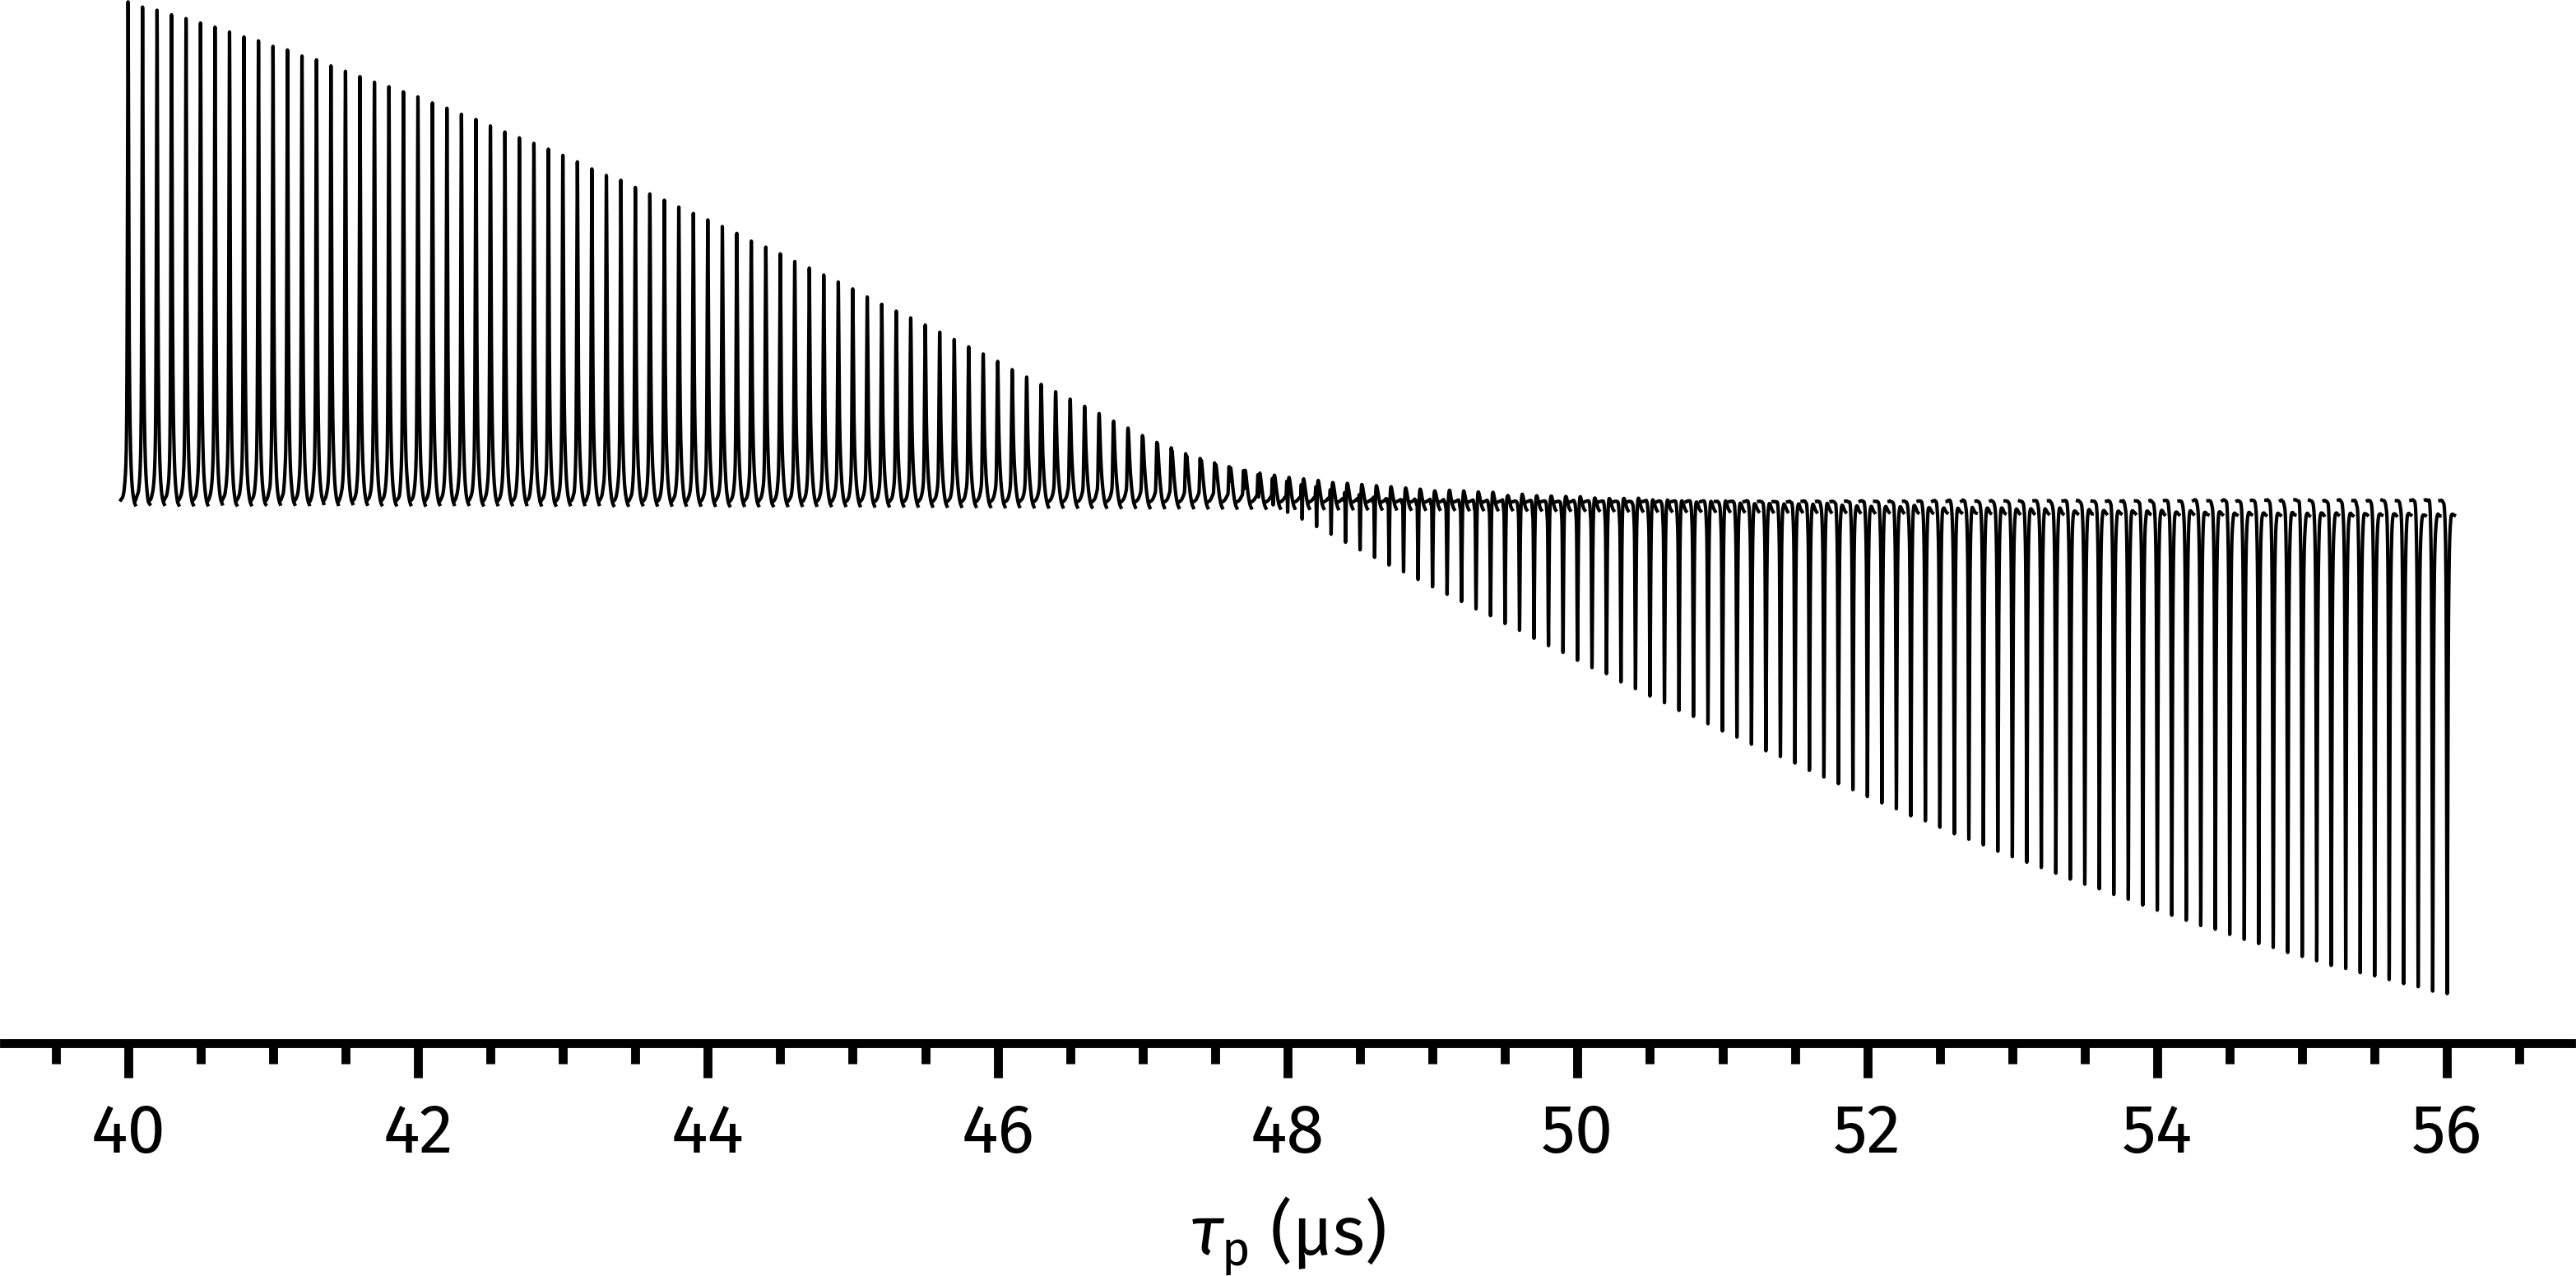
\includegraphics[]{poise/p1_scan_spectra.png}%
    \caption[Pulse width array]{
        An example of a pulse width array, where the variation of the water peak is monitored with changes in pulse width (the sample used in DMSO-$d_6$, but is slightly wet).
        These spectra were acquired manually; the TopSpin \texttt{popt} command would yield essentially identical results.
        \datacode{6F-200826}
    }
    \label{fig:p1_scan_spectra}
\end{figure}

TopSpin provides a built-in mechanism for measuring a pulse width array using the \texttt{popt} command.
The pulse--acquire spectrum is measured for pulse widths between a lower and upper bound, and the user specifies a spectral region of interest which \texttt{popt} uses to determine the null in spectrum intensity.%
\footnote{In fact, \texttt{popt} uses the notion of a cost function as well, in that it determines the point where the cost function is minimised. In this case, I set it to use the \texttt{MAGMIN} cost function, which seeks to minimise the intensity of the magnitude-mode spectrum; this is essentially identical to the \texttt{minabsint} cost function which was used for the POISE optimisations except that it only applies to the spectral region of interest.}
While this usually yields highly accurate results, the acquisition of so many spectra is relatively time-consuming and arguably unnecessary if the only purpose is to determine the null.

A more rapid method for pulse calibration is the nutation experiment of Wu and Otting\autocite{Wu2005JMR}, which allows the \ang{90} pulse width to be determined in a single-scan experiment.
In this experiment, an RF pulse with a given power level, corresponding to an (unknown) amplitude of $\omega_1'$, is applied during acquisition.%
\footnote{To be precise, it is applied for a proportion $d$ of the dwell time between acquisition of successive points in the FID; $d$ is called the \textit{duty cycle} and must be accounted for when calculating the pulse width using this method.}
Assuming that the pulse is applied along the $x$-axis, this leads to the following product operators during the acquisition period:
\begin{equation}
    \label{eq:pulsecal_operators}
    I_z \xrightarrow{\omega_1' t_2} I_z \cos(\omega_1' t_2) - I_y \sin(\omega_1' t_2)
\end{equation}
and an FID of
\begin{equation}
    \label{eq:pulsecal_signal}
    s(t_2) = -\sin(\omega_1't_2) = -\frac{1}{2\mi}(\exp(\mi \omega_1' t_2) - \exp(-\mi \omega_1' t_2)),
\end{equation}
which when Fourier transformed yields an antiphase doublet where the two peaks are separated by the frequency $2\omega_1'$.
Measuring the separation between the two peaks directly yields the unknown amplitude $\omega_1'$, from which $\taup' = \pi/(2\omega_1')$ can be calculated.
Typically, the RF amplitude $\omega_1'$ is rather smaller than the amplitude $\omega_1$ which we would like to apply the hard pulse at, and thus $\taup' > \taup$.
However, this can be adjusted for using the power levels applied (which are known to the user).

Although the nutation experiment can be performed extremely quickly using the TopSpin \texttt{pulsecal} command, often only requiring a few seconds, the pulse widths calculated are generally slightly shorter compared to the value obtained from a \ang{360} null.
This is a known effect which arises because the separation is calculated from the top of the peaks, which correspond to the most homogeneous region of the $B_1$ profile.\autocite{Wu2005JMR}
On the other hand, the \ang{360} null (as measured through \texttt{popt} or POISE, for example) measures a signal which is averaged over the entire $B_1$ profile.


\subsubsection{Optimisation results}

\begin{table}[!ht]
    \centering
    \begin{tabular}{ccccc}
        \toprule
        Entry & Method & Optimum found (\unit{\us}) & FEs & Time taken (\unit{\s}) \\
        \midrule
        1  & \texttt{popt}      & 48.40        & 41   & 299    \\
        2  & \texttt{pulsecal}  & 46.64        & --   & 37     \\
        3 & POISE (NM)         & 48.38        & 10   & 76--79 \\
        4 & POISE (MDS)        & 48.38        & 10   & 77--80 \\
        5 & POISE (BOBYQA)  & 48.29--48.41 & 6--7 & 46--54 \\
        \bottomrule
    \end{tabular}
    \caption[Comparison of methods for \ang{360} pulse width determination]{
        Comparison of methods for \ang{360} pulse width determination.
        \texttt{popt} grid searches were run between values of \qty{40}{\us} and \qty{56}{\us}, with a linear increment of \qty{0.4}{\us} (which, through interpolation, provides a precision of approximately \qty{0.2}{\us} in the result, matching the tolerance used for POISE).
        \texttt{pulsecal} was run as normal and the reported pulse width multiplied by 4 to obtain the \ang{360} pulse width for comparison.
        POISE optimisations were run according to the routine in \cref{tbl:poisecal_48}.
        \datacode{6F-200826}
    }
    \label{tbl:poisecal_48}
\end{table}

Compared to these two existing methods, we expect POISE to be faster than the \texttt{popt} grid search, and also more accurate than the nutation experiment in \texttt{pulsecal}.
This is borne out in practice (\cref{tbl:poisecal_48}).
\texttt{popt} yields an optimum of \qty{48.4}{\us}, which is closely matched by POISE.
However, across all five optimisation runs performed for each algorithm, POISE locates this optimum using far fewer FEs because its algorithms are more efficient than a simple grid search.
While the \texttt{pulsecal} routine is even faster than POISE,%
\footnote{It could be yet faster if it was instructed to not optimise the receiver gain prior to performing the nutation experiment.}
it underestimates the \ang{90} pulse width by about 4\%.
In this particular case, POISE is the only option which strikes a useful balance between speed and accuracy.
These results also provide the first evidence that Py-BOBYQA is generally faster than the simplex-based methods: this observation is consistently reproduced in many of the other optimisations in this chapter.


\subsubsection{Different initial points}

One question we might reasonably ask is how robust POISE is towards poor initial guesses.
In the case of the pulse width calibration, the answer is \textit{very} robust.
\Cref{tbl:poisecal_43,tbl:poisecal_53} summarise the results obtained with an initial guess of \qty{43}{\us} and \qty{53}{\us} respectively.
There is slightly decreased performance in that a few more FEs are required for convergence, but the accuracy of the result is unchanged.

\begin{table}[htb]
    \centering
    \begin{tabular}{ccccc}
        \toprule
        Entry & Method      & Optimum found (\unit{\us}) & FEs & Time taken (\unit{\s}) \\
        \midrule
        1 & POISE (NM)     & 48.38        & 14 & 109--114 \\
        2 & POISE (MDS)    & 48.38        & 14 & 108--112  \\
        3 & POISE (BOBYQA) & 48.27--48.33 & 9  & 70       \\
        \bottomrule
    \end{tabular}
    \caption[Pulse width calibrations using initial guess of \qty{43}{\us}]{
        Pulse width optimisations with an initial point of \qty{43}{\us}.
        The POISE routine is the same as in \cref{tbl:poisecal_48}, except with \texttt{"init":[43.0]}.
        \datacode{6F-200826}
    }
    \label{tbl:poisecal_43}
\end{table}

\begin{table}[htb]
    \centering
    \begin{tabular}{ccccc}
        \toprule
        Entry & Method      & Optimum found (\unit{\us}) & FEs & Time taken (\unit{\s}) \\
        \midrule
        1 & POISE (NM)     & 48.38        & 14 & 110--114 \\
        2 & POISE (MDS)    & 48.25--48.38 & 16 & 123--126 \\
        3 & POISE (BOBYQA) & 48.26--48.33 & 9  & 69--70   \\
        \bottomrule
    \end{tabular}
    \caption[Pulse width calibrations using initial guess of \qty{53}{\us}]{
        Pulse width optimisations with an initial point of \qty{53}{\us}.
        The POISE routine is the same as in \cref{tbl:poisecal_48}, except with \texttt{"init":[53.0]}.
        \datacode{6F-200826}
    }
    \label{tbl:poisecal_53}
\end{table}

It is tempting to use this example to draw the conclusion that the initial point does not matter in POISE optimisations.
However, this is only really true for a simple optimisation like this.
Looking again at the reference grid search in \cref{fig:p1_scan}, it is clear that there is no other possible minimum that the optimiser could converge to.
Furthermore, the noise in the cost function is almost indiscernible.
These represent the \textit{ideal} conditions for an experimental optimisation to work, and it is not surprising that extremely good performance is obtained with POISE.
Some of the subsequent examples include more difficult or more noisy cost functions.
We will see that POISE does indeed have \textit{some} tolerance towards poor initial points, even in the presence of noise (after all, this is the entire purpose of using derivative-free algorithms).
However, for very challenging optimisations (especially ones with many parameters) it is very likely that the optimisation will ultimately converge to a local minimum close to the initial point.
